\subsection{Positionsbestimmung}
UND FUNKTIONSWEISE


In diesem Kapitel wird zunächst einmal geklärt, was Positionsbestimmung ist. 
Nach Alex Küpper ist die Positionsbestimmung wie folgt definiert:

\begin{table}[h]
	\centering
	\begin{tabular}{|p{16cm}|}\hline
		\textbf{Zitat ?:} \glqq Positioning is a process to obtain the spatial position of a target \grqq  \cite[S.121]{Kuepper2005} \\ \hline
		\textbf{Übersetzung:} Positionsbestimmung ist ein Prozess, um die räumliche Position eines Ziels zu erhalten. \\ \hline
	\end{tabular}
\end{table}

Mit räumlicher Position ist hierbei ein Standort gemeint, der zu einem geeigneten Bezugssystem bestimmt wird. Das bedeutet ein Position der sich auf das Bezugssystem „Weltkarte“ bezieht repräsentiert den geografischen Standort auf der Weltkarte. Die Position mit dem Bezugssystem eines bestimmten Gebäudes repräsentiert den Standort in dem Gebäude. Bsp.: Stockwerk 1 Raum 139b.

Ein weiteres Zitat bezüglich der Positionsbestimmung grenzt den Begriff Positionsbestimmung deutlich von Ortung ab. Dieser Unterschied soll hier auch aufgezeigt werden. Hierzu das Zitat der Webseite www.itwissen.info:

\begin{table}[h]
	\centering
	\begin{tabular}{|p{16cm}|}\hline
		\textbf{Zitat ?:} \glqq Die Begriffe Positionsbestimmung und Ortung werden häufig synonym benutzt; sie unterscheiden sich allerdings im Detail. So wird mit der Positionsbestimmung der Ort von Objekten oder Personen eindeutig in einem geografischen Koordinatensystem festgelegt. Sie bildet die Basis für die Ortung und wird dann zur Ortung, wenn Dritten die ermittelte Position mitgeteilt wird. \grqq  \cite[Positionsbestimmung]{itwissen} \\ \hline
	\end{tabular}
\end{table}

Das Zitat ist aussagekräftig und grenz Positionsbestimmung und Ortung eindeutig voneinander ab.

In diesem Kapitel wird, wie es der Titel vorgibt, nur die Positionsbestimmung betrachtet. Dieser ist die Voraussetzung, um Ortung (die Übertragung der Position) überhaupt durchzuführen. Allerdings wird im weiteren Teil dieser Arbeit verstärkt die Ortung betrachtet werden. Die Übertragung der Position spielt nämlich zur Bereitstellung eines „location based Services“ in nahezu allen Fällen eine große Rolle. Da die Positionsbestimmung für die Ortung benötigt wird, diese hier im Detail vorgestellt.

TODO: Küpper S.123
Fundamentals ergänzen??

Bei einer Positionsbestimmung werden Messdaten gesammelt, um die eigenen Position festzulegen. Die Messdaten beziehen sich dabei immer auf festgelegte Fixpunkte, von welchen die Position schon bekannt ist.  Diese Daten sind zum Beispiel Winkel, Geschwindigkeit und Entfernung.

In den kommenden Kapiteln werden unterschiedliche Methoden/Techniken zur Positionsbestimmung aufgezeigt. Diese werden in drei Kategorien eingeordnet, die satellitengestützte Positionierung, Positionierung in Mobilfunknetzen und Positionsbestimmung in Gebäuden.

TODO: Robustheit ergänzen???

Kein Verfahren zur Positionsbestimmung ist perfekt. 
Deshalb werden die unterschiedlichen Methoden/Techniken zur Positionsbestimmung anhand von drei ?Qualitäts?-Merkmalen betrachtet. Diese werden hier kurz erläutert.

\begin{enumerate}
\item Bereich (Scope)\\
Ein Positionssystem ist immer auf einen Bereich bezogen, in dem eine Position theoretisch bestimmt werden kann. Dieser Bereich kann stark variieren von einem Raum bis zu einem weltweiten Bereich.\\
\longrightarrow Ein großer Scope ist besser
\item Abdeckung (Coverage)\\
Die Abdeckung eines Positionssystems kann maximal so groß sein, wie es der Bereich zulässt. Die Abdeckung ist die Teilmenge des Bereichs, in dem tatsächlich die Position bestimmt werden kann. So ist es beispielsweise bei einem Satellitenpositionssystem nicht möglich eine Abdeckung in Gebäuden oder unter der Erde zu gewährleisten.\\
\longrightarrow Eine große Abdeckung ist besser
\item Präzision (Precision)\\
Ein Positionssystem kann einen Standort nicht exakt, sondern mit einer gewissen Abweichung bestimmen. Diese Abweichung kann von Umwelteinflüssen abhängen und für eine Positionsbestimmung an der selben Stelle abweichende Ergebnisse liefern. Die Robustheit eines Positionssystem trägt somit zur Präzision bei. \\
\longrightarrow Eine höhere Präzision ist besser
\end{enumerate}
\cite[S.183]{Schiller2004}


\textbf{Satellitengestützte Positionierung}

Satellitengestützte Positionierung basiert, wie der Name schon vermuten lässt, auf Satelliten. 

Das bekannteste System zur satellitengestützte Positionierung ist das Global Positioning System, dass mit GPS abgekürzt wird. Auf GPS wird nach einer Erläuterung über das generelle Funktionsprinzip von Satellitenpositionierung eingegangen.

Gegeben für eine Positionsbestimmung sind Satelliten, die sich in der Erdumlaufbahn befinden und elektromagnetische Wellen auf die Erde funken. Damit eine Position auf der Erdoberfläche mit Hilfe von Satelliten errechnet/bestimmt werden kann, muss zuerst einmal ein Gerät vorhanden sein, dass die elektromagnetischen Wellen der Satelliten empfangen kann.

Ist das gegeben kann prinzipiell die Position des Nutzers auf der Erdoberfläche anhand von der exakten Position von mindestens drei Satelliten ($s_{n}$) und des Abstands zu diesen Satelliten ($r_{m}$) bestimmt werden.

\cite[S. 188]{Schiller2004}

Vergleiche hierzu Abbildung \ref{fig:Grundprinzip Satelliten}

\begin{figure}[h]
\centering
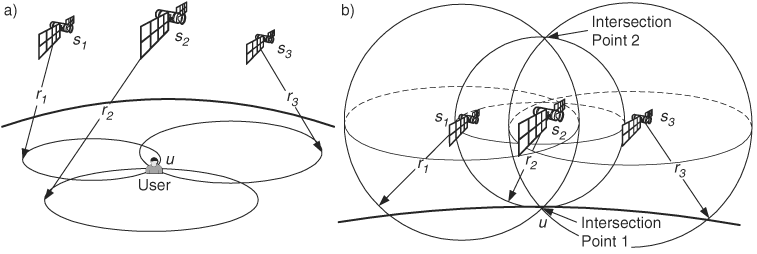
\includegraphics[width=0.99\textwidth]{ref/images/prinzip_satelliten.png}
\caption[Grundprinzip Satelliten Positionsbestimmung]{Grundprinzip Satelliten Positionsbestimmung}
\label{fig:Grundprinzip Satelliten}
\cite[S. 188]{Schiller2004}
\end{figure}

In Abbildung \ref{fig:Grundprinzip Satelliten} a) stellen die Kreise Positionen auf der Erde dar, an denen ein User-Position anhand des gemessenen Abstands ($r_{m}$) möglich ist. In dieser Darstellung mit drei Satelliten ist die User-Position eindeutig an dem Schnittpunkt aller drei Kreise. In Abbildung \ref{fig:Grundprinzip Satelliten} b) wird die Darstellung ins dreidimensionale überführt. Hierbei ist nun zu erkennen, dass die Kreise zu Kugeln geworden sind. Daraus resultierend gibt es nun einen zweiten Schnittpunkt. Für die Positionsbestimmung gibt es nun zwei mögliche User-Positionen. Dieses Problem beseitigt man einfach, indem man die logisch wahrscheinlichere Position als richtige ansieht. In der Abbildung wäre das Intersection Point 1, da Intersection Point 2 im Weltall liegt und davon auszugehen ist, dass sich Menschen auf der Erdoberfläche befinden.

Es wurde nun erläutert, wie sich die Position ermitteln lässt, wenn dem Nutzer die Position der Satelliten und der Abstand zu diesen bekannt ist. Wie diese Werte ermittelt werden wurde noch nicht erwähnt. Darauf wird nun eingegangen.

Satelliten Positionen:\\
Satelliten kreisen um die Erde. Sie sind also Ständig in Bewegung. 

\begin{figure}[h]
\centering
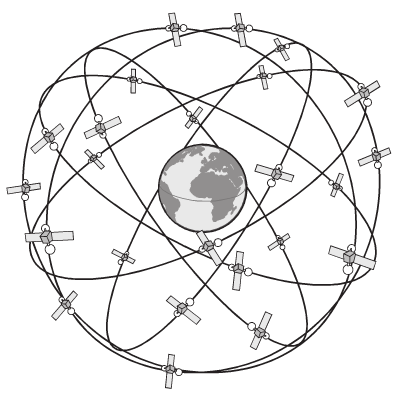
\includegraphics[width=0.4\textwidth]{ref/images/GPS_Umlaufbahn.PNG}
\caption[Umlaufbahn von GPS Satelliten]{Umlaufbahn von GPS Satelliten}
\label{fig:Umlaufbahn Satelliten}
\cite[S. 164]{Kuepper2005}
\end{figure}

Da sie in zuvor festgelegten Umlaufbahnen kreisen, kann die Position eines Satelliten abhängig von der Zeit errechnet werden. 
Diese Berechnung kann ohne Probleme auf einem Smartphone stattfinden. Die einzigen Daten die dazu nötig sind, ist eine aktuelle Uhrzeit, sowie die Satellitennamen mit der dazugehörigen Umlaufbahn. Solche Daten befinden sich standardmäßig auf GPS fähigen Geräten. Bei Bedarf, durch den Ausfall oder das Hinzukommen neuer Satelliten, werden diese Daten aktualisiert.


Abstand zu den Satelliten:\\
Der Abstand zu Satelliten wird anhand von der Zeit berechnet, die das Signal vom Satelliten bis zum Empfänger benötigt. Diese Zeit wird dadurch ermittelt, dass ein vom Satelliten die aktuelle Zeit gesendet wird. Sobald diese beim Empfänger ankommt wird der Zeitunterschied $ \bigtriangleup t $ zur aktuellen Zeit ermittelt. Da sich elektromagnetische Wellen mit Lichtgeschwindigkeit $ c $ fortbewegen, beträgt die Geschwindigkeit näherungsweise 300.000 $km/s$. Mit der Formel $ r = c \bigtriangleup t$ lässt sich dann die Entfernung zum Satelliten ermitteln. Das Verfahren funktioniert allerdings nur, wenn die Uhren vom Satelliten und des Empfängers exakt synchronisiert sind. 
\cite[S. 189]{Schiller2004}

Verfahren zur Uhren Synchronisation:\\
Eine Abweichung der Uhren von nur $1\mu s$ ergibt aufgrund der hohen Geschwindigkeit der elektromagnetischen Wellen eine Abweichung der bestimmten Position von ca. 300 Metern.
\cite[S. 189]{Schiller2004}

Jeder Satellit ist mit einer Atomuhr ausgestattet um immer die richtige Zeit zu senden. Eine Atomuhr in ein Smartphone einzubauen macht allein schon aus wirtschaftlicher Sicht keinen Sinn. Deshalb muss es ein Verfahren geben, mit dem die Uhren synchronisiert werden könne, oder der Unterschied zwischen den Uhren bestimmt werden kann.

Das Grundprinzip dieses Verfahrens wird nun erläutert. Dazu werden zunächst einige Variablen definiert.

$ t_{s} $ steht für die Systemzeit des Satelliten, an der das Signal gesendet wurde.

$ \tilde{t}_{s = t_{s} + \delta t_{s}} $ ist die Zeit des Satelliten unter Berücksichtigung der Abweichung $ \delta t_{s} $ zur exakten Zeit.

$ t_{u} $ steht für die Systemzeit der Users, zu der er das Signal empfangen hat.

Die Systemzeit des Users kann eine Abweichung zur exakten Zeit haben. Deshalb wird für die weitere Betrachtung $ \tilde{t}_{u = t_{u} + \delta t_{u}} $ unter Berücksichtigung der Abweichung $ \delta t_{u} $ zur exakten Zeit verwendet.

$ \bigtriangleup \tilde{t} = \tilde{t}_{u} - \title{t}_{s} $ ist die gemessene Zeit zwischen dem Abschicken des Signals vom Satelliten bis zum Empfang des Signals beim User.

$ c $ gibt die Lichtgeschwindigkeit an.

Im Abschnitt \glqq Abstand zu den Satelliten \grqq wurde schon die Formel zur Berechnung des Abstands $ r = c \bigtriangleup t $ erwähnt. Diese basiert allerdings darauf, dass beide Uhren synchronisiert sind.

Hier wir diese Formel dahingehend angepasst, dass die Abweichungen $\bigtriangleup t$ von den Systemzeiten berücksichtigt werden. Das ist dann der gemessen Abstand $p$:

\glqq 
\begin{align}
p &= c * \bigtriangleup \tilde{t} \\
  &= c * (\tilde{t}_{u} - \tilde{t}_{s}) \\
  &= c * ((t_{u} + \delta t_{u}) - (t_{s} + \delta t_{s})) \\
  &= c * (t_{u} - t_{s}) + c * (\delta t_{u} - \delta t_{s}) \\
  &= r + c * (\delta t_{u} - \delta t_{s})
\end{align}
\grqq \cite[S. 190]{Schiller2004}

Die Systemzeit des Satelliten ist bei dieser Betrachtung als exakt anzusehen, da Satelliten mit einer Atomuhr ausgestattet sind und von Bodenstationen kontrolliert werden. $\delta t_{s}$ ist damit als 0 anzusehen.

Daraus erhalten wir $p = r + c * \delta t_{u}$

$r$ kann hierbei durch die Koordinaten des Satelliten und des Users dargestellt werden: $p = \sqrt{(s_{x} - u_{x})^{2} + (s_{y} - u_{y})^{2} + (s_{z}-u_{z})^{2}} + c * \delta t_{u}$

Diese Gleichung enthält nun vier unbekannte Variablen $u_{x}, u_{y}, u_{z} und \delta t_{u}$. 

Um diese Gleichung zu lösen benötigt man diese vier unbekannten Variablen. Jeder dieser Variable kann selbst wieder über eine Gleichung bestimmt werden. Um alle vier Gleichungen zu lösen sind dann vier Satelliten nötig. 

Es gibt nun mehrere Möglichkeiten diese Lösung anzugehen. Es kann zum Beispiel durch ein Näherungsverfahren geschehen. Herr Schiller verweist in deiner Arbeit dabei auf die Möglichkeit eine Taylor Reihe.

Da es ab dieser Stelle nur noch eine mathematische Aufgabe ist die Lösung zu finden, und es dafür wiederum unterschiedliche Ansätze gibt, wird darauf nicht weiter eingegangen.
\cite[S. 190]{Schiller2004}


\underline{GPS}

Das Global Position System wurde vom Amerikanischen Verteidigungsministerium entwickelt. Es gibt eine Variante, die nur dem Militär zugänglich ist und eine, die der Zivilbevölkerung frei zur Verfügung steht. 

Das GPS System besteht auf 24 Satelliten, die um die Erde kreisen. Die Satelliten können über Basisstationen, die auf der ganzen Erde verteilt sind, ihre Uhren synchronisieren und ihre richtige Umlaufbahn beibehalten. 
\cite[S. 162]{Kuepper2005}


\begin{figure}[h]
\centering
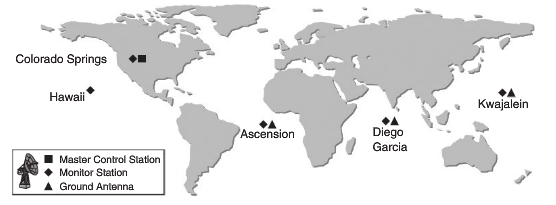
\includegraphics[width=0.99\textwidth]{ref/images/GPS_Basisstation.PNG}
\caption[GPS Basissationen]{GPS Basissationen}
\label{fig:GPS Basissationen}
\cite[S. 163]{Kuepper2005}
\end{figure}

Das GPS basiert grundsätzlich auf den zuvor vorgestellten Mechanismen zur Standortbestimmung. 

Es gibt allerdings einen Unterschied in der militärischen und der zivilen Variante. Die militärische Variante bietet eine höhere Präzision, steht allerdings nur Ländern die der NATO angehören zur Verfügung. 

Die zivile Variante bietet im Normalfall eine fast so hohe Präzision, wie die militärische, kann aber von der U.S. Army durch einen Mechanismus, der Selective Avaulability (SA) heißt deutlich ungenauer gemacht werden.

Vergleiche hierzu Abbildung \ref{fig:GPS Praezision}.

PPS steht für die militärische Variante wohingegen SPS für die zivile Variante des GPS steht.

\begin{figure}[h]
\centering
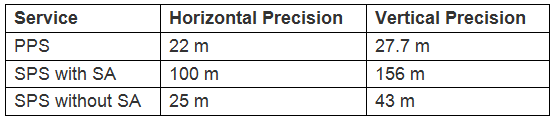
\includegraphics[width=0.6\textwidth]{ref/images/GPS_Praezision.PNG}
\caption[GPS Präzision]{GPS Präzision}
\label{fig:GPS Praezision}
\cite[S. 195]{Schiller2004}
\end{figure}

Die Präzision von GPS kann durch Differential GPS nochmals verbessert werden. Dazu wird in einer Basisstation, zu der eine exakte Position vorhanden ist, die GPS Position ermittelt. Gibt es Abweichungen durch die Atmosphäre wird von der Basistation eine Korrektur erstellt, die dann an den User weitergeleitet werden kann, um auch dessen Präzision zu verbessern.

Vergleiche hierzu Abbildung \ref{fig:DGPS}
\begin{figure}[h]
\centering
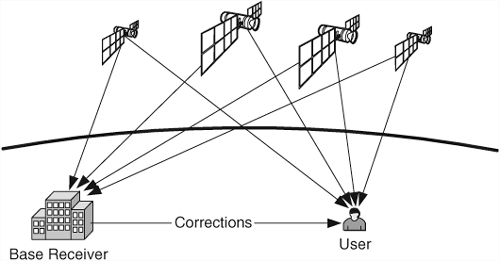
\includegraphics[width=0.99\textwidth]{ref/images/DGPS.PNG}
\caption[Präzision Differential GPS]{Präzision Differential GPS}
\label{fig:DGPS}
\cite[S. 196]{Schiller2004}
\end{figure}

Betrachtet man Satelliten Positionierung und im speziellen GPS kann man für die Qualitätskriterien die folgende Bewertung abgeben.

\longrightarrow Bereich (Scope) Prinzipiell ist eine Standortbestimmung auf der ganzen Welt möglich.

\longrightarrow Abdeckung (Coverage) Die Position kann überall auf der Erdoberfläche, mit einer Ausnahme, der Positionsbestimmung in Gebäuden, bestimmt werden. Das bietet eine sehr große Abdeckung.

\longrightarrow Präzision (Precision) Eine hohe Präzision wird durch viele Satelliten und Korrektursignale ermöglicht. Die Position ist so  robust gegen Umwelteinflüsse.

\cite[S. 187]{Schiller2004}

Die Kosten zum Betreiben von Satelliten sind immens hoch. Es gibt allerdings auch andere Positionierungssysteme, die auf vorhandene Funknetze setzen. Diese werden nun vorgestellt.

\textbf{Positionierung in (Mobil)Funknetzen}

GSM

190 Länder. In Gebäuden und außerhalb verfügbar. Nicht in dünn besiedelten Gebieten, wie Bergen oder das offene Meer. 
\longleftrightarrow großer Bereich (Überall Funktmasten installiert werden können.
\longleftrightarrow Abdeckung sehr flächendeckend. sogar in Gebäuden.

Verschiedene Ansätze der Positionsbestimmung. Unterscheidung liegt in Präzision. 

MPS mobile positioning system von Ericsson

- Cell of Globar identify
- Segment antennas
Bild zur Erklärung (vielleicht selber zeichnen
- Timing advance
Figure 7.9
-Uplink Time of Arrical 
Figure 7.9

\cite[S. 206 - 209]{Schiller2004}


\textbf{Positionsbestimmung in geringer Abdeckung}

Beispiel Gebäude, da dort andere Positionierungssysteme versagen (GPS)

Auf zwei Methoden wird eingegangen. Erst auf Positionsbestimmung anhand von WLAN Netzwerken. Danach auf Radio Beacons.

WLAN Netzwerke
Gebäude mit vielen WLAN AccesPoints ausgestattet. 
Position kann anhand der Signalstärke zu den Accespoints ermittelt werden.
Dazu kann man ein Verfahren von Microsoft verwenden, welches auf Messwerten basiert. Table 7.2

Problem an dem Verfahren ist, dass wenn zu wenig Accespoints vorhanden sind, wird die Position schnell ungenau. Außerdem sind Messerung zum Konfigurieren erforderlich. Ein alternativer Ansatz wäre Triangulation.

Radio Beacons
Seite 203


\textbf{GPS, Mobilfunk, WLAN, Bluetooth}

\subsubsection{Kriterien für die Standortbestimmung}
Genauigkeit, Bestimmungszeit, Robustheit


\subsubsection{Arten der Standortbestimmung}
GPS, Mobilfunk, WLAN, Sterne, Beacons